\subsection{ISO/SAE 21434: Overview}\label{subsec:iso-sae-21434}

The ISO/SAE 21434 standard is a joint standard developed by the International Organization for Standardization (ISO) and the Society of Automotive Engineers (SAE) to address the cybersecurity of road vehicles.
The standard is designed to provide a framework for the development of secure vehicles and their components.
The standard covers the entire lifecycle of a vehicle, from design and development to production and operation.
It provides guidelines for identifying and assessing cybersecurity risks, as well as for implementing security measures to mitigate those risks.
The standard also includes requirements for monitoring and responding to cybersecurity incidents, as well as for managing the security of vehicle components and systems.
The ISO/SAE 21434 standard is intended to be used by vehicle manufacturers,
suppliers, and other stakeholders in the automotive industry to improve the cybersecurity of vehicles and protect them from cyber threats\cite{iso-correlation}.

\textbf{ISO/SAE 21434} is the international standard designed to address cybersecurity in road vehicles, particularly focusing on electrical and electronic (E/E) systems.
Released in August 2021, this standard establishes guidelines for original equipment manufacturers (OEMs) and suppliers to manage cybersecurity risks throughout the entire lifecycle of vehicle systems.
Moreover, it introduces the concept of Cybersecurity Assurance Levels, which categorize the severity of cybersecurity threats and the corresponding measures to mitigate them\cite{moukahal2021towards}.
\subsubsection{Key Points}\label{subsubsec:key-points-1}

\begin{enumerate}
    \item \textbf{Cybersecurity Culture}:
    \begin{enumerate}
        \item Promotes a strong cybersecurity culture within organizations, emphasizing safety and security in all engineering processes.
    \end{enumerate}

    \item \textbf{Risk Management}:
    \begin{enumerate}
        \item Provides guidelines for identifying and managing cybersecurity risks, including threat analysis, impact assessment, and risk mitigation strategies.
    \end{enumerate}

    \item \textbf{Documentation Requirements}:
    \begin{enumerate}
        \item Establishes a series of required work products, including asset identification, threat scenarios, and a cybersecurity incident response plan.
    \end{enumerate}

    \item \textbf{Lifecycle Integration}:
    \begin{enumerate}
        \item Covers cybersecurity from the initial design phase to decommissioning, ensuring that security measures are integrated throughout the vehicle's lifecycle.
    \end{enumerate}

    \item \textbf{Collaboration with Other Standards}:
    \begin{enumerate}
        \item Works in conjunction with existing standards, particularly ISO 26262 (which focuses on functional safety), ensuring that both safety and security are considered during vehicle development.
    \end{enumerate}

    \item \textbf{Continuous Monitoring and Improvement}:
    \begin{enumerate}
        \item Encourages continuous cybersecurity assessment and updates to address evolving threats and vulnerabilities.
    \end{enumerate}
\end{enumerate}

\subsubsection{Correlations}\label{subsubsec:correlations}

\begin{enumerate}
    \item \textbf{ISO 26262}: Emphasizes the relationship between safety and security, ensuring that both aspects are addressed in vehicle design.
    \item \textbf{UNECE WP.29 R155}: Provides a legal framework for cybersecurity in vehicles, complementing ISO/SAE 21434 by outlining regulatory requirements and compliance timelines.
\end{enumerate}

\subsubsection{Limitations}\label{subsubsec:limitations}

\begin{enumerate}
    \item \textbf{Lack of Specific Technical Solutions}:
    \begin{enumerate}
        \item The standard does not prescribe specific technologies or methods for implementing cybersecurity measures, potentially leading to varied interpretations and implementations among manufacturers.
    \end{enumerate}

    \item \textbf{Potential for Fragmentation}:
    \begin{enumerate}
        \item Without defined methods, companies may adopt proprietary solutions that could create compatibility issues within a highly connected automotive environment.
    \end{enumerate}

    \item \textbf{No Mandatory Compliance}:
    \begin{enumerate}
        \item ISO/SAE 21434 is a guideline rather than a regulation, meaning compliance is not enforced by law, which could lead to inconsistent application across the industry.
    \end{enumerate}

    \item \textbf{Limited Focus on Cybersecurity Techniques}:
    \begin{enumerate}
        \item While the standard outlines processes and documentation, it does not provide detailed methodologies for specific cybersecurity assessments or techniques to evaluate vulnerabilities effectively.
    \end{enumerate}
\end{enumerate}

\subsubsection{Cyber Threats}\label{subsubsec:cyber-threats}

\begin{enumerate}
    \item \textbf{Threat Analysis and Risk Assessment}:
    \begin{enumerate}
        \item The standard emphasizes conducting thorough threat assessments to identify potential vulnerabilities in vehicle systems and the likelihood of cyberattacks.
    \end{enumerate}

    \item \textbf{Incident Response}:
    \begin{enumerate}
        \item Requires the establishment of a cybersecurity incident response plan to ensure quick and effective actions are taken in the event of a security breach.
    \end{enumerate}

    \item \textbf{Continuous Improvement}:
    \begin{enumerate}
        \item Advocates for regular updates and improvements to cybersecurity practices to adapt to new and emerging threats in the automotive landscape.
    \end{enumerate}
\end{enumerate}

\subsubsection{Conclusion}\label{subsubsec:conclusion}

ISO/SAE 21434 aims to enhance the cybersecurity posture of the automotive industry by establishing a comprehensive framework for managing risks associated with E/E systems in vehicles.
While it addresses critical aspects of cybersecurity, its limitations, particularly the lack of prescribed technical solutions and mandatory compliance, highlight the need for continued development and adaptation to effectively mitigate evolving cybersecurity threats.

\subsection{UNECE WP.29: Overview}\label{subsec:unece-wp-29}

The United Nations Economic Commission for Europe (UNECE) oversees regulations concerning cybersecurity and software updates for road vehicles, specifically through the UNECE WP.29 framework.

\subsubsection{Key Points}\label{subsubsec:key-points}
\begin{enumerate}
    \item \textbf{Cybersecurity Regulations (R155)}: Established in March 2021, these regulations are crucial for OEMs and Tier suppliers in UNECE member countries.
    Compliance is mandatory for new vehicle types since July 2022 and for all vehicles from July 2024.
    \item \textbf{Components of R155}:
    \begin{enumerate}
        \item \textbf{Cybersecurity Management System (CSMS)}: Organizations must implement a CSMS to manage cyber risks across the vehicle lifecycle.
        This systematic approach involves defining processes, responsibilities, and governance to protect vehicles from cyber threats.
        \item \textbf{Certification}: OEMs must apply for a Certificate of Compliance for their CSMS, which is valid for three years, subject to renewal.
        The approval process involves assessments and validation by technical services and Approval Authorities.
    \end{enumerate}
\end{enumerate}

\subsubsection{Threats and Mitigations in R155}\label{subsubsec:threats-and-mitigations-in-r155}
\begin{enumerate}
    \item \textbf{Annex 5 Structure}:
    \begin{enumerate}
        \item \textbf{Part A}: Identifies 32 potential threats related to various attack surfaces (e.g., communication channels, back-end servers).
        Each threat includes examples of vulnerabilities affecting Confidentiality, Integrity, and Availability (CIA) of vehicle systems.
        \begin{enumerate}
            \item \textbf{Confidentiality Threats}: For example, eavesdropping on communications.
            \item \textbf{Integrity Threats}: Unauthorized manipulation or deletion of vehicle data.
            \item \textbf{Availability Threats}: Risks such as Denial of Service (DoS) attacks that may compromise user safety.
        \end{enumerate}

        \item \textbf{Part B}: Outlines high-level mitigation actions specifically for vehicle-related threats.
        For instance, to protect confidential data in transit, one suggested mitigation is to ensure that all confidential communications are safeguarded, although it does not detail specific implementations.

        \item \textbf{Part C}: Addresses threats from external entities, such as back-end servers.
        It recommends measures like applying security checks and adhering to OWASP guidelines to prevent unauthorized access.
    \end{enumerate}
\end{enumerate}

Overall, the UNECE regulations emphasize a comprehensive and systematic approach to cybersecurity in the automotive sector, requiring OEMs to be proactive in identifying risks and implementing suitable mitigations.


\subsection{Comparative Analysis}\label{subsec:comparative-analysis}
\begin{figure}[!htb]
    \centering
    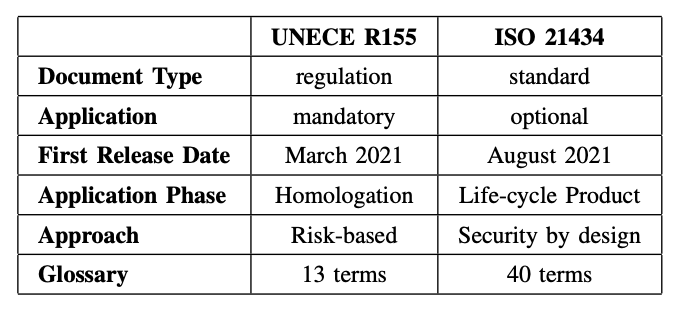
\includegraphics[width=0.7\linewidth]{figures/diff-standards}
    \caption{Comparison of ISO/SAE 21434 and UNECE WP.29 R155}
    \footnotesize{From \cite{comparison-standard} }
    \label{fig:comparison}
\end{figure}

The development of UNECE R155 and ISO/SAE 21434 arose from the need to enhance cybersecurity in road vehicles to ensure user safety and protect personal data.
Although UNECE R155 was released in March 2021 and ISO/SAE 21434 followed in August 2021, the two documents serve different purposes within the automotive cybersecurity landscape.
Here’s a detailed analysis of their similarities, differences, and limitations.

\subsubsection{Similarities}

\begin{enumerate}
    \item \textbf{Common Objectives}: Both UNECE R155 and ISO/SAE 21434 aim to improve cybersecurity throughout the product lifecycle of road vehicles, enhancing user safety and data protection.

    \item \textbf{High-Level Solutions}: Both documents propose high-level solutions and do not prescribe specific implementations, allowing manufacturer flexibility to adopt suitable measures for their contexts.
    \begin{enumerate}
        \item \textbf{Threat Identification}: UNECE R155 identifies possible threats, such as malicious internal messages, while ISO/SAE 21434 cites similar scenarios requiring analysis and mitigation.
    \end{enumerate}

    \item \textbf{Structured Organization}: Both documents require a structured approach to managing cybersecurity, including
    \begin{enumerate}
        \item Cybersecurity Management Systems (CSMS) and risk identification.
        \item Continuous monitoring and improvements, supported by internal or external audits.
    \end{enumerate}

    \item \textbf{Risk Mitigation}: Both documents emphasize risk mitigation processes, where UNECE R155 focuses on risk management and ISO/SAE 21434 outlines specific risk treatment options (e.g., avoiding, reducing, sharing).

    \item \textbf{Documentation for Compliance}: Documentation required for ISO/SAE 21434 can support compliance with UNECE R155, facilitating a cohesive approach to managing cybersecurity.

    \item \textbf{Continuous Review}: Both documents mandate the ongoing revision of cybersecurity practices and documentation throughout the vehicle lifecycle, ensuring ongoing support and updates.

    \item \textbf{Cost Considerations}: Both UNECE R155 and ISO/SAE 21434 acknowledge the need for cybersecurity compliance that balances implementation costs with operational feasibility, highlighting the complexity of the automotive environment.
\end{enumerate}

\subsubsection{Differences}

\begin{enumerate}
    \item \textbf{Type of Document}:
    \begin{enumerate}
        \item \textbf{UNECE R155}: A legally binding regulation that mandates compliance for all UNECE member countries.
        \item \textbf{ISO/SAE 21434}: A non-mandatory standard expected to be widely accepted within the automotive industry.
    \end{enumerate}

    \item \textbf{Implementation Timeline}:
    \begin{enumerate}
        \item \textbf{UNECE R155}: Compliance was mandated for new vehicle types from July 2022 and for all vehicles by July 2024.
        \item \textbf{ISO/SAE 21434}: Became applicable from August 2021.
    \end{enumerate}

    \item \textbf{Application Phases}:
    \begin{enumerate}
        \item \textbf{UNECE R155}: Focused primarily on the homogenization phase, requiring documentation for getting a Certificate of Compliance for the CSMS.
        \item \textbf{ISO/SAE 21434}: Encompasses the entire product lifecycle, requiring ongoing documentation for annual audits, from design to decommissioning.
    \end{enumerate}

    \item \textbf{Glossary Size}:
    \begin{enumerate}
        \item \textbf{ISO/SAE 21434}: Contains a comprehensive glossary with over three times more definitions than UNECE R155, which aids in clarity and understanding of cybersecurity terminology.
        \item \textbf{UNECE R155}: Lacks detailed definitions, potentially leading to varied interpretations of terms like \textit{confidential data}.
    \end{enumerate}

    \item \textbf{Threat and Mitigation Approach}:
    \begin{enumerate}
        \item \textbf{UNECE R155}: Provides tables outlining specific threats and recommended mitigations.
        \item \textbf{ISO/SAE 21434}: Does not directly address attacks but emphasizes vulnerability analysis and risk assessments.
    \end{enumerate}

    \item \textbf{Detail of Compliance Requirements}:
    \begin{enumerate}
        \item \textbf{UNECE R155}: Offers a less detailed list of compliance documentation compared to ISO/SAE 21434, which specifies required work products in detail.
        \item \textbf{ISO/SAE 21434}: Details the attack feasibility ratings and their implications in Annex G, emphasizing the importance of selecting appropriate methods for risk-based decisions.
    \end{enumerate}

    \item \textbf{Regulatory Authority}:
    \begin{enumerate}
        \item \textbf{UNECE R155}: Enforced by regulatory authorities in UNECE member states, with compliance being mandatory.
        \item \textbf{ISO/SAE 21434}: Lacks mandatory enforcement, relying on industry acceptance and best practices.
    \end{enumerate}
\end{enumerate}

\subsubsection{Conclusion}\label{subsubsec:conclusion2}

In conclusion, while UNECE R155 and ISO/SAE 21434 share common goals of enhancing cybersecurity in the automotive industry, they differ significantly in their nature, application, and requirements.
UNECE R155 is a binding regulation focused on approval, while ISO/SAE 21434 serves as a comprehensive standard for the entire vehicle lifecycle.
Their complementary nature allows manufacturers to leverage the documentation and processes of one to meet the requirements of the other,
fostering a more robust approach to cybersecurity in road vehicles\cite{comparison-standard}.
The problem remains that the lack of mandatory enforcement in ISO/SAE 21434 could lead to inconsistent implementation across the industry and potentially undermine the standard's effectiveness in addressing cybersecurity threats.